

%TODO - short paragrah introducing the general background idea

This chapter outlines the major contributions leading to the current state of art for Software Defined Networks. 
This area is marked by three phases: the introduction of programmable network hardware; the control and data plane separation; and, finally the de facto standardization of the data plane interface. 
We will cover selected papers from the last two phases that have most influence to work. 
For an overview of all the existing work we redirect the read to the paper by Feamster et. al, \cite{},  


%TODO - section History covers the historical path of the data and control plane separation starting at a routing systems and culminating in SDN. 

Software Defined Networks (SDN) changed the traditional model of network architecture and design. 
%FIXME - bad phrase  
Traditionally, networking  relied and evolved over a non-transparent distributed model for
the deployment  of  protocols and configuration of devices. 
This model lead to complex protocols and management functions. 
SDN presents a new way of thinking in networking, shifting the complexity of protocols and management functions from  the  networks devices to a general purpose logically centralized service. 

Historically  the network academic environment has followed an  ad-hoc approach to networking where protocols are introduced as a response to specific problems. 
Scoot Shenker, a networking researcher from Berkley\footnote{Scoot Shenker has played a fundamental role in SDN development, collaborating in many papers. He is also co-founder of both ONF \cite{onf} and Nicira Networks - both very important to SDN.}, ironically sums up  this contribution to networking as a ``big bag of protocols'' \cite{Shenker:2011ys}. 
In his opinion there is a lack of \emph{control abstractions} in current network architectures that in alliance  with  their  distributed nature, leads to the  complex infrastructure available today. 
Additionally the network field has failed to developed the appropriate tools for managing such complexity. 

%FIXME - move to intro
SDN breaks this complex model through the physical detachment of the control and data planes.  
The motivation behind this decoupling is the following: if the distributed network state can be collected and presented to a logically centralized service then it is simpler to both to specify network level objectives as well as to translate these objectives into the appropriate configuration of network devices. 
These planes, when loosely coupled, can simplify the development of protocols and the management of network infrastructures. 


\section{Software Defined Networks}
\glsresetall
\label{sec:background:sdn}

\subsection{General Architecture}

\subsubsection{Architecture}
In March 2011 the Open Network Foundation was created with the
participation and support from several industry partners \cite{onf}. ONF  is a ``non-profit consortium
dedicated to the transformation of networking through the development
and standardization of a unique architecture called Software-Defined
Networking (SDN)''. They have done so, by releasing a white-paper
defining the design principles for a SDN architecture and the
advantages of it \cite{ONF:2012ui}. They are also responsible for the standardization
process of the OpenFlow protocol.

It is important to emphasize that Software Defined Networks is not a
standard. It should be
clear, by now, that SDN's are an architectural pattern with two
essential properties:

\begin{itemize*}
\item Decoupling of the control plane from the data plane;
\item The network control must be driven by software.
\end{itemize*}

In this section we present the SDN architecture used as reference throughout this document.  

\subsubsection{General architecture.} The architecture of Software Defined Network is presented in Figure
\ref{fig:sdn-stack}. A bottom up explanation of the responsibilities of
each layer follows:

\begin{figure}
  \centering 
  \footnotesize
  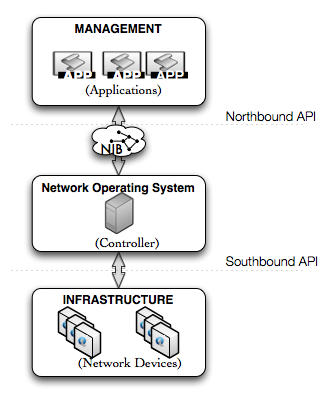
\includegraphics[scale=0.5]{pic/related/sdn-stack.png}
  \caption[SDN Architecture]{\textbf{SDN Architecture}: is composed by three
    layers: in \textbf{Management} resides the application
    logic that governs the overall network behavior; The
    \textbf{Control Plane}   allows the integration
    of  Management applications and exposes an interface for the
    manipulation of the network (northbound API). It also exposes the Network
    Information Based (NIB); Finally the network is
    represented in the \textbf{Infrastructure} layer. The devices must
  implement an interface allowing configuration (southbound API)}
  \label{fig:sdn-stack}
\end{figure}

\begin{itemize}
\item[] \textbf{Infrastructure Layer:} In this layer are the network
  devices responsible for packet forwarding. Any device 
  can be used (wireless access point, Ethernet switch, router) as long as it implements 
  a standard configuration interface (e.g., OpenFlow). Throughout the text we refer to all these devices as switches;
\item[] \textbf{Network Operating System (NOS):} Provides a standard
  interface to the upper layer (i.e., the northbound interface) allowing the manipulation of the network
  state such as forwarding tables in the managed devices. The
  configuration of devices is actually done by the NOS by interaction
  with the Infrastructure interface for configuration (i.e., the southbound interface). Additionally, it should provide features
  for the integration of Management layer applications.  Throughout
  the text we use NOS, controller or control plane to refer to this
  layer;
\item[] \textbf{State Distribution: } 
\item[] \textbf{Management:} This is where the network logic operates. In this layer
  resides the definition of network level objectives in the form of
  one or more applications. These applications interact with the NIB
  to consult and modify the network state. 
\end{itemize}


\subsubsection{Types of Controllers.} The controller is often
categorized in the literature
``logically centralized'' \cite{Gude:2008jd,Greenberg:2005boa}. This concept is used in distributed systems literature
to refer to a physically distributed system that appears, to
its users,  as a
coherent and  transparently distributed service (i.e., it does not
appears to be distributed). The term is perhaps
not well employed in SDN literature as pointed out in
a blog post, by Martin Casado, a Stanford researcher and Nicira
co-founder \cite{:zr}. We will not maintain
this terminology either. Instead, we define that the control platform is 
either  \textbf{distributed} or 
\textbf{centralized} for the remaining discussion. In the centralized
case a single controller is responsible for all the network
Infrastructure as opposed to the distributed case where several
controllers are used.

Another category  distinction in controller software is based on another text
from Casado and Koponen \cite{Martin-Casado:2011ly}, where
three categories of controllers are discussed: 


\begin{itemize}
\item[] \textbf{Single Purpose Controller:} lack support for general management
  applications. Ethane is an example of this type of controllers; 
\item[] \textbf{Thin Controller:} present a northbound interface that is
  strongly-coupled to the southbound interface. Most controllers fall
  under this category. Usually these controllers are known as OpenFlow controllers given the use of OpenFlow in the southbound interface.  
\item[] \textbf{General Controllers:} offer a general purpose service with loosely
  coupled south and northbound interfaces. Transition from the OpenFlow protocol for
  other protocol may  be completely transparent to the Management layer.
\end{itemize}


\begin{itemize}



\item This reactive model is not ideally. One could also have a proactive model where network changes are applied to the data store view,  resulting (possibly) in configuration changes to the data plane. But typically requirements for the network view are event driven, for example, the location of hosts with OpenFlow is limited to listening and processing packet-in events for flow requests that did not match a flow in the switch table. Typically the installed flow rules to access a host expired on a time basis and/or usage based. This serves two purposes: first it recycles the switch flow tables such that it does not lead to exhaustion of the switch hardware capabilities, but also allows applications to refresh the devices location which can be essential in mobility scenarios caused by mobiles users, virtual machine migration or others. 
But by reverting this tendency to a proactive model with more device drivers (e.g., snmp or others) to access the servers we can avoid this behaviour and have an proactive model whereby the traffic that reaches the controller can possibly decrease in magnitude. Data center measurements suggest that 
\end{itemize}

\subsection{Evolution}

\subsubsection{RCP}

\begin{itemize}
\item PARAGRAFO - Tal fez coiso. Coiso  decouplou para resolver vários problemas existentes no ibgp que é tal e coiso. A year later coiso. 
\begin{itemize}
  \item  In 2004 Feamster et. al.  \cite{Feamster:2004tg} published an paper described the architecture of \gls{rcp}.
  \item Establishes one of the first decoupled approaches to network management. 
  \item Decoupled the control plane from the data plane to centralize it only for routing. 
  \item This work addressed problems in the \gls{ibgp} protocol, used between peers inside an \gls{as} to distribute external routing information. 
  \item  This protocol is a fundamental in the Internet. \gls{bgp}  
  \item  Has been implemented a year later by Caesar et. al.  \cite{Caesar:2005wsa}
\end{itemize}

\item PARAGRAFO - Problemas que o césar identificou
  \begin{itemize}
  \item Cesar lists the scalability limitation of full mesh configuration in \gls{ibgp} and the inconsistency problems of route reflectors as the majors problems in \gls{ibgp} architectures. 
  \item  Indeed, the full mesh configuration by operating with %\BigO{$n^2$} network connections (and associated protocol state) between $n$ routers, challenges the scalability of the network. 
  \item Likewise, the route reflection technique used to mitigate the scalability problem imposes an hierarchy structure between routers that limits their vision of the entire routing state. As a result, this technique can lead to routing problems such as route oscillations and forwarding loops (in some cases persistent).  
  \end{itemize}


\item PARAGRAFO RCP solves this with a logically centralized control plane that maintains a  global network state, of the routing state, in spite of operating  with $n$ connections (for $n$ routers).  
  \begin{itemize}
  \item  Manages the routing decision process instead of routers. 
  \item  It scales for two reasons : lower number of connections, and specialized domain data structures that save memory to keep the route state. 
  \item It is correct because the control plane has an complete view of the routing information. 
  \end{itemize}

\item PARAGRAFO \gls{rcp} is distributed for reliability. 
  \begin{itemize}
  \item Each router connects to more than one server. 
  \item It is able to operate even in the presence of network partitions, and avoids a single point of failure. 
  \end{itemize}

\item PARAGRAFO Interestingly, the authors proof that an \gls{rcp} does not requires more than an eventually consistent protocol in order to operate correctly. 
  \begin{itemize}
  \item In this context operate incorrectly means that different \gls{rcp} replicas assign different routes to an router.
  \item The authors are able to proof this, since they assume both that they can identify a steady state on the routing protocol (where all route information has been delivered to the \gls{rcp} replicas. 
\item Additionally they also assume that replicas, only assign routes  for routers in a partition for which they have full routing information (both exterior and interior). 
\item As such, and as point out by the authors, lack of a consistency protocol 
  \end{itemize}

This scheme introduces the possibility of inconsistency since  \gls{rcp} replicas have different views of the network. 
And different replicas could install conflicting rules in the same router. 
The authors show in the paper that there is no need to have consistency protocols between \gls{rcp} replicas to prevent such conflicts. 
This does not affects the safety of their system given that it is designed such that each replica makes routing decisions only for the partitions for which it has a complete interior topology view. But for the same reason it can affect liveness since each since different RCSes may fail to assign routes to routers. 
We note that this is proof takes the assumption that the replicas have already converged to what the authors name a steady ``state''  where the progation of route updates has already converged in the \gls{rcp} replicas. 

\item It is paradoxically that this same work who is partially motivated by problems caused by lack of consistency in the network state that is distributed across routers ends up being eventually consistent in the state distribution plane. 
\end{itemize}

\subsubsection{4D}


\begin{itemize}
\item  PARAGRAFO - \gls{rcp} is great but is focused on a single control function (routing). There needs more. 
  \begin{itemize}
     \item In 2005, Greenberg et. al., published a seminal paper that proposes a clean slate architecture to address the (arguably) root problems of existent architectures. 
     \item Identify the root problem of existent architectures. 
     \item The authors arguments is manifold. But it rooted in the complexity manifested from twisting the control and data plane in the same hardware. 
  \end{itemize}


The proposed architecture is based on three fundamental principles: specification of  global network level goals (e.g., routing, security policy);  centralization of the entire network state (e.g., topology, link state) and finally; direct control of the underlying network devices. 

\item Paragrafo sobre as 4 layers do 4D

%4 layers
\item Named 4D due to the 4 planes of this architecture. 

\begin{itemize}
\item[] \textbf{Decision:}  defines network-level goals and 
  translates them to configuration primitives of the network
  equipment. This plane maintains a representation of the current state of the network (i.e., the network view); 
\item[] \textbf{Dissemination:}  connects the Decision and Data plane. Must be
  done with robustness guarantees; Is independent of the data plane network guarantees. 
\item[] \textbf{Discovery:} provides discovery information (e.g., network
  equipment, interfaces, etc.) from the Data plane to the Decision plane; Discover physical components in the network. 
\item[] \textbf{Data:}  is governed by the network equipment
  infrastructure. Provides packet forwarding functions and implements
  an interface to the Decision plane;  
\end{itemize}


The 4D project [34] advocated four main layers—the data plane (for processing packets based on configurable rules), the discovery plane (for collecting topology and traffic measurements), the dissemination plane (for in- stalling packet-processing rules), and a decision plane (consisting of logically centralized controllers that con- vert network-level objectives into packet-handling state). 
% 4 layers 

\item\gls{rcp} focus in control the \gls{bgp} routes only. But 4D envisions global control over all data plane forwarding mechanisms (e.g., FIB entries, packet filters, NAT's, tunnels, packet scheduling and buffer management) that should be available as a unifed  resourced to satisfy network goals. 



The 4D architecture, even without a concrete implementation,   presented a significant mark in the history of SDN by setting the  ground for discussion and evolution focused on this essential  decoupling of control and data planes.  PASSAR PARA O RCP. 

% \item  The origins of SDN as an architectural principle for networks can be traced back to the 4D architecture published in  2005 that ``generated both broad consensus and wide disagreements from
% the reviewers''  \cite{Greenberg:2005boa}. In this seminal work the authors identify essential
% problems governing  the traditional network architecture and  present an
% explanation of the design process behind a clean-slate architectural
% pattern for network management and innovation.  

%TODO - root problem is coupling of control plane with data plane. 
%TODO - results in the lack of way to specify network wide goals
%TODO - management goals are decomposed in ad-hoc manual scripts distributed by the data plane infrastructure. 

% The authors identify  the root cause of the complexity inherent to the classic Internet design as the  entanglement  of control and forwarding functions in the network devices. They advocate that this complexity is tied to the lack of accessible control abstractions in the network devices. 

% 4D effectively removes network logic  from the Data plane
% responsibilities. It advocates that what was previously done through complex
% routing protocols and per-box configurations (e.g., security policy
% definitions)  can be specified in the Decision plane. 

\subsubsection{Ethane}

\begin{itemize}
\item Particular expansion of the 4D project following footprints. 
\item Casado et. al. present in 2007  \cite{Casado:2007kb}
\item Ethane \cite{Casado:2007kb} was published in 2007 and presents a
network architecture for the enterprise with emphasis in
security. 


\item WHY DOES HE DO IT
\item Decoupling the control plane from the central plane. Multiplexing network elements functionality into one.  (SEE PREVIOUS PHRASE TO MAKE SURE PEOPLE UNDERSTAND). 

\item Follows the lead of 4d . identifies the problem as being manual configuration that results into errors. 
\item Focused in making the entreprise network architecture more manageable by centralized 


\item WHAT DOES HE DO? 
\item INTRODUCE CONTROLLER as the server. 
\item In Ethane the controller plays the interposition role between any any two pair of hosts.  SO packets only flow through the network if he decides to do so. 
\item  In addition it is constantly aware of the identity of the hosts by maintaining ``the location of all users and machines, and authenticating all names and address''. HE can alaways associate a packet with a particular user or host. 




THE CONTROL PLANE : 
\item (equivalent to the 4D decision plane), maintains a global network view (topology, authenticated users, hosts and address binding, policy, registration of users)
\item The controller manages network objectives focused in security. In the paper two objects are clearly defined:  ``the network should be governed by policies declared over high level names'' (i.e, the network policy does is not confronted with the low level and dynamically allocated addresses);  and  the ``policy should determine the path that packets follow''.  (i.e., finer grained control) ; ``the network should enforce a strong binding between a packet and its origin''. 
\item In Ethane the 4D Decision plane  is instantiated in a complex software
running in a server named \emph{controller}. The controller guarantees
that the security policy is respected. To do so, it can manipulate the network
devices available in the network. 
The security policy is defined over
high-level names. As authentication is performed in the controller it is easy to maintain
bindings between these names and dynamic addresses. 

THE DATA PLANE : 
\item In Ethane the switches are dumb. ``reduced to a flow tables machines that are populated by the controller based on high-level security policies''
\item They do not perform thypical control operations (e.g., learn addresses, forwarding tables, ACLS or NAT, routing protocols)

\item The devices perform  flow-based
forwarding  with the help of a local  flow table that is maintained by the
controller. Every flow that fails to match with any of the rules
available in the flow table  is redirected to the controller. After the
control logic is applied the controller may perform several actions
including: forwarding/flooding the packet;  installing flows in the
switch;  drop the packet; etc., 
\item They built the're own switches (in NETFGPA programmable switch platforms and in software). 

\item BIGGEST CONTRIBUTION 
\item Because, at the time, scalability and resilience were standard objections to a centralized approach (as proposed by 4D and Ethane), their 
\item Biggest contribution is the results from a practical deployment. 
\item Ethane major contribution comes from the practical  experience with
the deployment in the Stanford University  campus network. 
\item Where a single prototype used was able to confortably handle a network of approximately 300 hosts. Furthermore, 
\item the  authors argue that a single desktop computer alone could handle a network with over 20K hosts. 


\item DISTRIBUTED AND CONSISTENCY
\item Distributed control, resilience and scalability are a common theme throughout the Ethane paper. 
\item We again see the discussion  for distributed control for improving resilience in the control plane. In Ethane. And in additions scalability.

\item The authors  DIVAGAM different modes for this distribution. In the primary-backup mode there is an active controller while other standby to take over its place in the event of failure. 
In this mode the standby controllers can keep slow-changing state (such as configuration and user registration) consistently while the binding information that associates network devices to users is kept under eventual consistency semantic. The only problem identified in the paper with this mode is that in the event of failures some users may need to reauthenticate. 
In contrast in the active mode, the two or more active Controllers take over the network. The authors envision that switches can balance their requests across these different controllers. Under this mode the authors argue that  the use of eventually consistency semantics for replication is sufficient in most implementations. Also they state that to solve conflicts in this data replication the use of consistency aware data structures such as convergent data structures or simple partitioning schemes (e.g., separate \gls{ip} address space across controllers for \gls{dhcp} allocation that is conflict free). Albeit arguing for eventual consistency they do state that is a need for further study and stronger consistency guarantees as the \gls{smr} can be employed when desired. 

\item (MAKE SURE THIS YOUR OPINION), we do not disagree, but we also do not agree. 
\item We believe that in a sensible environment motivated by a EXAGERADO security policy it is crucial that the distribution of the control plane must be dependable. 
\item IFF we must be sure that the security is to be respected in every single communication. 
\item Off course due to the asynchronous nature of a network (i.e., as soon as you install a rule in a switch, the network wide policy or topology may already have changed)  we need more than a stronger and dependable distributions mechanisms in the control plane. Indeed we need to expand this strong semantics to the data plane (which is covered in Section~\ref{sec:relatedWork:consistentPlane}.) 

\end{itemize}



\subsubsection{OpenFlow}
 %BAD PHRASE
INTRODUCTION 
Both Ethane \cite{Casado:2007kb} and 4D \cite{Greenberg:2005boa}
focused in the decoupling of the control plane from the data plane, however there is also required that the control plane can programatically define the data plane configuration. 

\begin{itemize}
\item The decoupling was established as solid architectural principle, but there was the lack of an standard interface on network devices. 
For general development of SDN  it is  necessary that a
standard interface is available. OpenFlow \cite{openflow}, published
in 2008,  was the first protocol enabling this interface by allowing
the remote manipulation of flow based forwarding network devices. 

\item OpenFlow (OF) is introduced in the context of an architecture similar to
Ethane \cite{Casado:2007kb}, in which network devices 
are also simple flow-based forwarding equipments 

\item WHAT DOES IT DO.
\item programmable hardware lowers the barrier to inovate. 
\item Generalize the behaviour. Instead of ip based , \gls{of} can define forwarding behavior on traffic flow based on 13 different packet headers. 
\item A router is ip, a switch is mac and a firewall is (ip, port and transport protocol), network address translators. 
\item ``Generalizes rules installations techniques'' 

\item  Enable a wide range of controller applications

DETAILS 
\item A flow
table resides in the network device and is composed of tuples
$\langle match,action \rangle$. The $match$ entry allows the device to match
arriving packets, while  $action$
specifies the forwarding behavior. Matches can be performed against
standard fields in Ethernet, IP and transport headers while actions can
range from dropping packets; forwarding to single port(s); and/or forwarding to controller. 


\item As in Ethane, a non-matching flow is usually forwarded to the controller who in
turn should instruct  the network device on future behavior through
the modification of the device flow table. Once the table is instructed, 
subsequent packet with matching headers can be forwarded without
the controller interaction. 


\item WHY IS IT GOOD. 
\item OpenFLow leverages on existent switch hardware. 
\item Based on capabilities already existent in the hardware
\item ``(Specifically fine-grained access contrl and flow monitoring)''
\item It became as easy as performing an firmware upgrade. 
\item Where previous as failed, OpenFlow succeed becoming defacto. 
\item So, SDN reasearch and industry community rapidly converged on using the OpenFlow. 
\item looking for ways to conduct exmperimental work on ``clean-slate'' network architectures 
\item So the data plane interface become immediately standardized. 
\item Become immediately deployable .

NOT PERFECT BUT WE USE IT. 
\item OpenFlow is not perfect \cite{OpenFlowNeedsYou} 
\item Still we consider only OpenFlow in our study. However we expect it to be orthogonal.
\item CITE ALTERNATIVES

Currently the OpenFlow specification is maintained by the Open Network
Foundation (ONF). At the time of writing, the version 1.3 \cite{of13} is available with
several improvements over the original paper \cite{openflow}. 

We cover OpenFlow in more detail later. Namely we give an brief overview of the fundamentals  that are required to understand the evaluation of our design. 

\end{itemize}
\item ``Whenever a switch sees a flow's first packet, because there is
  no flow entry configured on the switch's flow table to match this
  flow, the first packet will be forwared to the controller. We call
  this packet a ``flow request''. The controller runs user defined
  applications to process a flow request, for example the controller
  computers a path for this flow and installs flow entries on every
  switch along the chosen path, so that subsequent packets of this
  flow can be handled by the switches locally. Finally the flow requet
  packet itself is sent back to the origin switch'' 


% From openflow.1.3.spec \cite{openflow-spec}
% Timeouts : (specified in flow\_mod messages). 
% idle timeout - `` If set and the \texttt{hard\_timeout} is zero the entry must expire after \texttt{idle\_timeout} seconds with no received traffic. ''
% hard timout  - ``if set the entry must be expired in the specified number of seconds regardless of whether or not packets are hitting the entry. A value of 0 means that a timeout has not been set''
% %``If the idle_timeout is set and the hard_timeout is zero, the entry must expire after idle\_timeout
% % seconds with no received traffic. If the idle\_timeout is zero and the hard_timeout is set, the entry
% % must expire in hard_timeout seconds regardless of whether or not packets are hitting the entry. If both
% % idle_timeout and hard\_timeout are set, the 
% % ow entry will timeout after idle_timeout seconds with
% % no trafficc, or hard_timeout seconds, whichever comes first. If both idle\_timeout and hard\_timeout are
% % zero, the entry is considered permanent and will never time out. It can still be removed with a flow_mod
% % message of type OFPFC\_DELETE.''

% OpenFlow: flowmod and flow removed FIXME 
% Maybe talk a little about the asynchronous problems and lacks of guarantees. 
% \begin{table}[ht]
%   \centering
%   \begin{tabular}[ht]{lll}
%     Match Fields &  Instructions & Timeouts \\ \toprule 
%     source MAC = 10:20:. \emph{AND}  protocol = ICMP  & port 2,3 & 5,10 ms \\ 
%     source IP = 10.0.0.0/24  & port 1 &  0/0 \\
%     source IP = 10.0.0.0/24 \emph{AND} protocol = TCP & controller & 0/0 \\ 
%     any & controller & 0/0 \\ \bottomrule 
%   \end{tabular}
%   \caption{Simplified representation of a flow table in OpenFlow switches }
  
% \end{table}


% \begin{itemize}
% \item Not event the first packet must go to the controller
% \item Wide array of matching. By default each packet is set to a match any . Bitmask masking if supported by the switch (notice the 10.0.0.0/24). 
% \item We use an explicit message, but table misses can also be configured to be forwarded to the controller. 
% \item wide range of instructions , including multi processing with the use of different flow tables. For our purposes it suffices to understand that we can control the forwarding process with commands as  forward or drop . In the table we only show example that forward the flow to different ports, including an example that forwards it to two different ports. 
% \item Hard timeout and idle timeout

% \end{itemize}

% \begin{itemize}
% \item Controller to switch communication. 
% \item ``Interface that connects each OpenFLow switch to a controller .  Through this interface, the controller configures and manages the switch, receives events from the switch , and sends packets out the switch'' 
% \item Over TCP 

% \item Controller to switch
%   \begin{itemize}
%   \item Messages that are initiated by the controller and may or may note rquire a response from the switch. 
% \item Modify state : manage state on the switch and add, delete and modify flow entries in  the OpenFlow tables. 
%   \item Packet-out messages used by the controller to send specific messages out a port. 
%   \item Barrier messages to ensure message dependencies have been met or to receive notifications for completed operations. 
%   \end{itemize}
% \item Asynchronous messages 
%   \begin{itemize}
%   \item Packet-in transfer the control of a packet to the controller. For all packets forwarded to the controller reserved port using a flow entry or the table-miss flow entry. This message contains at least the headers of the data plane message that causes it. In some cases the entire message is sent. Throughout the text we abuse the language and use  the data plane event to refer the packet-in message received at the controller. For example we might say: the controller receives an \gls{ip} request when in practice it receives a packet-in request triggered by an \gls{ip} request at the switch. 
%   \item Flow-removed inform the controller about the removal of a flow entry from a flow table. 
%   \end{itemize}

% \end{itemize}


% Message handling
% \begin{itemize}
% \item Provides reliable message delivery and processing, but does not automatically provide acknowledgements or ensure ordered message processing;
% \item It is built over \gls{tcp} but it can not ensure message ordering because multi connections can be open to enhance parallelism; 
% \item Messsages are guaranteed eventual delivery unlesss the channel fail; unless the OpenFlow channel fails entirely, in which case the controller should not assume anything about the switch state (e.g., the switch may have gone into ``fail standalone mode'' ) 
% \item Ordering can be ensured through the use of barrier messages. in the absence of barrier messages, switches may arbitrarily reorder messages to maximize performance; hence controllers should not depend on a specific processing order. 
% \end{itemize}

% \begin{itemize}
% \item The OpenFlow channel supports multi controllers connectivity
% \item The hand-over between controllers is entirely managed by the controllers themselfes.
% \item A controller can operate in one of three modes : 
% \item In the master mode it has full access to the switch. The switch ensures that only one controller is responsible for this role.  When a controller change its role to master the previous controller is immediately changed to the slave role. 
% \item In the slave role the controller only has read-only access to the switch and by default does not receive switch asynchronous messages (except the port status messages that are triggered by changed in the a particular port status - up or down). If this controller attempts to modify the switch state (e.g., flow  modification message) then the switch will reply with an error message
% \item Finally the equal role is identical to the master role , but several controller may have it. 
% \item Any controller in any role can specify what kind of switch asynchronous messages are received in the controller and which ones it does not cares about. 
% \item There is a master identifier to identify how many times the mastership has changed. It is a monotonically increasing counter. When changing a role, the controller must specify an id in the request that is greater than the currently counter seen at the switch, otherwise the message is discarded

% \item The switch must be configured at startup with the ip address of the switch. 
% \item In case the switch looses connection to all controllers it can enter the fail secure mode or fail standalone mode. In te first the only change is that packets destined to the controller are dropped. Timeout entries are eventually dropped. In the second the switch behaves as a legacy Ethernet switch or router. 
% \item On reconnection the flow entries remain. 

% \end{itemize}


\subsubsection{The Network Operating System (NOX)}

In Ethane this
feature was presented in a monolithic  implementation of the controller.

\subsubsection{Network Operating}

\begin{itemize}
\item After \gls{of} 
\item Nox and Maestro. Concurrently introduced in 2008 . 
\item The Network Operating System (NOS) terminology  was initially used in the
context of Operating Systems (OS's) to name OS's with network services available. In the
context of SDN it was, to our knowledge,
introduced by Gude et al. \cite{Gude:2008jd} and
Cai et al. \cite{Z.-Cai:2008fk}.
\item Observe and control a network. 
\item Conceptual decomposition of the control plane into two layers. 
\item Analyzed the control plane and establish techniques and decomposition of this plane. 
\item NOX establishes that the Network View shared between applications, managed by the control plane. 

\item Nox establishes the view of a pipeline whereby different applications process the packets from the data plane. 


\item FUNCTIONS
\item Abstract the interaction with the switches. In this sense \gls{of} is equivalent an device driver in a regular \gls{os}. More controller-to-data-plane solutions are possible.  This is an interface to the entire network. 

\item Manage the interaction between applications. Coordination, isolation, etc., 
\item 
\item ``More generally, the emergence of a network operating system offered a conceptual decomposition of network operation into three layers [47]: (1) a data plane with an open inter- face; (2) a state management layer that is responsible for maintaining a consistent view of network state; (3) control logic that performs various operations depending on its view of network state. Although the development of the OpenFlow protocol itself was mostly an engineering effort, efforts to drive adoption have also produced several contributions''
\item The role of the Network Operating System is to provide applications residing above it the ability to effectively control and observe the state of the network. This ability is provided through a programmatic interface defined in the Network Operating System itself and should be general enough to support a broad spectrum of  network management applications. With the help of this interface it is easier to define and deploy network control applications such as firewalls and load balancers. 

EXPAND HOW DOES IT WORKS
\item Both NOX and Maestro isolate state to share information between different applications. 
\item Nox is focused on providing higher level of abstractions so they need not deal with low level details. It later expanded this vision an general, distributed controller framework (see Section \ref{sec:related:onix}). 

\item Maestro orchestrate the control decisions made by various management applications. It later focused in the parallelizing the performance of a controller \ref{sec:related:maestro.})  

\item This functionality of a NOS is similar to conventional  Operating Systems (OS's) with the fundmental difference of the managed resources. A regular OS manages hardware devices from a computer  and  a NOS manages a network. The latter environment is harder to manage than the former.  Aside this difference, the role of the NOS is to implement the device drivers to communicate with the network devices and also provide a platform for deployment of network control applications with integration, communication and isolation features (as a regular OS does for computational systems). 

\item  In essence, this concept set a clear line in the separation of network applications from configuration of network devices. The NOS abstraction brings different attributes to the development process of network control functionality that, until now, was bound by the hardware and respective software development cycle. Development is still bounded due to the capabilities of the devices under management of the NOS but at least the NOS itself and the applications can follow a software-only
development cycle. Additionally one can expect most of SDN functionality to be heavily dependent   on the applications build on top of NOS much like current  OS user level functionality is offered by applications running outside the kernel.

%TODO - they can be a challenge to distributed controllers. 


\item Both NOX and Maestro have come to influence most open source controllers existent today. This event oriented mechanisms to support different applications that work in cooperation to contribute to the wide established networks goals. 

\end{itemize}


% \end{itemize}
% \subsubsection{OpenFlow}


% \section{Physically Centralized  Controllers}
% \glsresetall
% \label{sec:background:centralized}


% In this section we present an overview of relevant centralized
% controllers. Centralized controllers are, by our definition, control
% planes that do not show any explicit support in the deployment of a
% different controllers processes over onde or more servers. 
% \subsection{Existent Controllers}
% %TODO - what defines a centralized controller. 
% %TODO - pipeline as a common model
% %TODO - event based
% %TODO - thin. 
% \subsubsection{NOX}
% \label{sec:nox}

% %TODO - move to network operating system 
% Network Operating System
% %TODO make references to section of network operating system 
% \begin{itemize}
% \item ``Focused on the network operating systems providing an uniform and centralized programmatic interface to the entire network''
% \item ``Analalogous to the read and write access to various resources provided by the computer operating systems, a network operating systems provides the ability to observe and controll a network''
% \item ``Does not manages the network itself; it merely provides a programmatic interface . Applications implemented on top of the network operating systems perform the actual management tasks.''
% \item This interfaces provides the core of a controller. Applications belong to the management layer whereby decisions that affect the switch state is done. The core just affects the controller state (the network view). 
% \item Openflow can be seen as a device driver to be used by the network operating system. 
% \end{itemize}

% NOX
% \begin{itemize}
% \item Network view.  Could be distributed with standard replication techniques (unspecified) for resilience; 
% \item ``The network view contains switch-level topology; the locations of users, hosts, middleboxes and other network elements; and the services (e.g., HTTP or NFS )  being offered but does not include the current state of network traffic;''
% \item According to the authors this choice of observation granularity provides adequate information for many network managements tasks and changes slowly enough that it can be scalably maintained in the network; 
% \item The choice of flow limits the control application in kind. It can't easily do deep packet inspect for example as it would hinder scalability too much; 
% \item ``In terms of consistency; the only network state that is global (i.e., must be used consistently across the controller processes) is the network view; this consistency requirements arises because applications use data from the network view to make control decisions, and those decisions should be the same no matter to which controller instance the flow has been sent. In constract, since neither packet state nor flow state are part of the network, they can be kept in local storage (i.e., packet state in switches, and flow state in controller instances).'' 
% \item The netowrk view is a set of indexed hashtables, with extensions for distributed access with local caching to aid scaling across multiple controller instances. 
% \item ``Thus, NOX applications should only write to it when a change is detected in the network, and not for every received packet'' 

% \item Reactive. Event based.   Pipeline based 
% \item The core controller has applications that maintain a switch and host level topology in the network view. Other applications include: discovery of network services, user and host authentication, network policy enforcement, and detect network scanning. 
% \item ``Some events are generated directly by \gls{of} messages such as switch koin, switch leave, packet received, port up/dow, and statistics received'';;
% \item set of handlers, registered to execute when a particular event handles. Even handlers are executed in order of their priority.
% \item Each handlers decides if the event should go further in the pipeline or not
% \item Applications handle events and trigger events also. 
% \item ``Each service is coupled with an associated event that can be leveraged by other applications''. 


% \item It is very intersting to see that the Nox authors consider that NOX can easily scale since the events affecting the network view are in the order of tens of events per second for networks of thousands of hosts. ``The global data structure, the network view, changes slowly enough that it can be maintained centrally (or for resilience, it can be kept consistently on a small set of replicas) for even very large networks'' 
% \end{itemize}


% NOX \cite{Gude:2008jd}  was published and publicly released under
% GPL in 2008. It was both developed in C++ and Python. NOX enables a standard interface for the integration of  Management applications 
% in the controller. These applications control
% network objectives and also cooperate to define the current
% network view (i.e., the NIB). The view is shared between applications. One of the
% contributions of the article was the definition of the Network
% Operating System abstraction for the controller service. However, NOX
% is a Thin Controller. 

% \begin{figure}
%   \centering 
%   \footnotesize
%   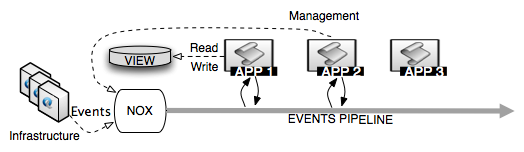
\includegraphics[scale=0.5]{pic/nox-pipeline}
%   \caption[NOX pipeline] {\textbf{NOX pipeline} An overview of the NOX
%     pipeline used for event processing by the Management applications. NOX
%   receives events that have originated either in the Infrastructure of
% the Management layer and dispatches them through a pipeline of
% applications who have registered for processing these events. 
%  As an example: \emph{PACKET\_IN} is a network event while
% \emph{USER\_AUTHENTICATED} could be an application event.}
%   \label{fig:nox-pipeline}
% \end{figure}

% NOX is a component framework with primitives for
% construction and deconstruction of OpenFlow
% based messages. The programming model is event-based. Applications (the components) are registered in a
% priority based pipeline with event handlers associated to either
% OpenFlow or applications events. This process can be seen in Figure
% \ref{fig:nox-pipeline}, which describes the NOX dispatching behavior. Notice
% that applications decide if the event should continue to be processed
% by the pipeline. NOX  currently ships
% with several applications (e.g., forwarding, topology discovery, host
% tracking, spanning tree, layer two switch behavior, etc.).

% NOX is a centralized controller  but the authors argue that it can easily be distributed for resilience if the shared state (the \emph{view}) is consistently distributed. 
% Initially it was a single threaded application not focused on
% performance. However, from its publishing date 
% several improvements have taken place
% \cite{Tootoonchian:2012uia,zen-doc-thesis} that have significantly improved
% NOX performance. Under the set of improvements we highlight the
% natural evolution to a multi-core aware application
% that statically distributes network requests to different threads. 

% In the time of writing, NOX is publicly available but has ramified into
% two different applications: A C++ based controller available in
% Linux and a Python  based controller (POX) available for
% several environments \cite{nox}.

% \subsubsection{Maestro}
% \begin{itemize}
% \item ``In general operating systems can be sseen as revolving around two basic purposes: providing applications with a higher level of abstraction so they need not deal with low-level details, and (ii) controlling the interactions between applications. Maestro focuses on the second , ``orchestrating" the contrl decisions made by various management applications''
% \end{itemize}

% Performance , fairness 
% \begin{itemize}
% \item Focused in fair service from the controller to the switches requests. while achieving the maximum performance requirements (low request handling and scalability on multi core processors
% \item ``We investiage what software design strategies would optimize the eprformacen of a controller machine under the workload characteristics of OpenFlow; assuming the hardware is a commodity computer based on a modern multi-core processor architecture''
% \item Otpimizing performacen requires a balancen between fairness, latency, and throughput 
% \item The controlelr must be able to run multiple copies of user applications in parallel to scale up throughput on multi-core processors and must do so while maintaining fairness and controlable latency.
% \item Users of the system must have the option to write simple single-threaded applications and leave it to the controller to parallelize them. 
% \item Found that the round-robin design achieves far superior and near optimal fairness while having excellent scalability, second only to the dynamic partition design. 
% \item Also present a workload-adapative request batching algorithm that automatically selects the granularity for batching requests for improved throughput while ensuring request handling latency is well controlled. 
% \item NOX and BEacon both statically assign the request from a fixed subset of the network switches to each worker thread. This design maximizes parallelism and is conceptually ideal when requests are uniformly arriving from all switches. 
% \item Maestro shows that even under a uniform workload from the swithces, not all worker threads run at exactly the same rate in practice, leading to a performance bias towards some switches. When not uniform, this design suffers from poor fairness and potentially suboptimal throughput due the under-utilization of some worker threads. 
% \item Maestro shows that while NOX and Beacon can achieve impressive raw aggregate throughput, as expected such a static batching strategy laeds to unnessarily large request handling latency when the system is under heavy load. 


% \item Maestro dynamically creates multiple worker threads, to work on multiple instances of the parallelized application. Furthermore it can stall pending application instances until the update of the shared network state is updated. 
% \end{itemize}

% \begin{description}
% \item[Shared-Queue] A select thread to read the incoming requests from the switches without blocking; Afterwars the requests are put inside a queue shared by all worker threads. One of the workers fetches the requests and leads him through the pipeline until completion;
% \item[Maestro-Static-Partition] Adresses the previous design by statically distributing each (or groups of ) switch socket to a different thread. This removes the need for synchronization in the shared queue design; This is the model followed by both NOX and Maestro 
% \item[Maestro-Dynamic-Partition] Improves by measuring the switch recent input rates and dynamically arranging the workers-to-switch-sockets binginds. This improves the system since a static partition model does not takes into account that different switches can impose different workloads on the controller 
% \item[Round Robin ] Each worker thread is individually running a round-robin service loop among all switch sockets. Each flow request is processed entirely by one of the worker threads, 
% \end{description}

% \begin{itemize}
% \item Found that round robin achieves the most balanced performance for the Controller but stays second best in throughput scalability. The first is dynamic partition but at the cost of increased delay. 
% \item Interesting analysis and complete study of the tradeoffs. But it may be that this parallel model is not well adapted to some controller requirements. It is not clear for instance if switches events can be processed out of order. For instances two successive events considering the state of a port are better handled in \emph{First-In-First-Out} (FIFO) sequence). But not even the \gls{of} standard specifies this clearly. 
% \item This also does not take into consideration the impact of blocking calls made by the worker threads to remote services that have an impact of latency. 
% \end{itemize}

% Maestro is the undergoing work of Zeng Cai covered in
% \cite{maestro}. It is presented as a Network Operating System focused
% in coordination and isolation of the applications  that control the
% infrastructure layer. Cai recognizes that Management components do not
% operate independently and in isolation. Instead, they operate
% concurrently with inter-dependent state (present in the NIB). With this in mind
% it aims to exploit parallell computing benefits in the control plane. 

% Maestro splits the regular pipeline execution such that it can
% be concurrently executed. As seen in Figure \ref{fig:maestro-pipeline} events may
% follow different execution paths since singular control components are
% not interested in every single event. Thus, Maestro can manage to
% execute several applications concurrently. However, in order to
% coordinate the control component access to the NIB Maestro opts to
% have a more granular network state model. The author argues that it is
% common to control components to be  interested only in  subsets of the
% NIB. In order to employ concurrent execution Maestro requires that
% applications specify  what subsets of the NIB they require as input
% and what subsets they modify as output. 

% Maestro employs
% coordination of the  execution of the applications with performance in
% mind. As an example based on Figure \ref{fig:maestro-pipeline} if the routing table
% (subset of the NIB) is updated while the RouteFlow application is running, then
% Maestro makes sure that the application will use the old version of
% the RoutingTable.

% \begin{figure}
%   \centering 
%   \footnotesize
%   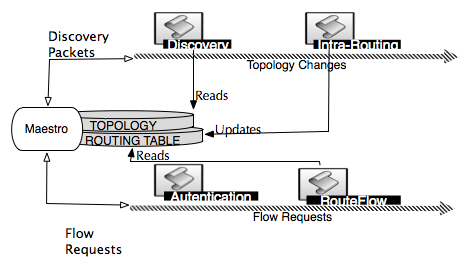
\includegraphics[scale=0.5]{pic/maestro-pipeline.png}
%   \caption[Maestro pipeline]{\textbf{Maestro pipeline} Maestro split the pipeline execution
%   into several concurrent pipelines based on the events applications
%   process and the state they access or modify. In the figure we can
%   see two execution paths: \textbf{Topology Changes} processes the
%   events triggered by changes in the Infrastructure and \textbf{Flow
%     Requests} processes new flow events.}
%   \label{fig:maestro-pipeline}
% \end{figure}


% The fundamental objective of Maestro is to maximize scalability in a
% centralized control plane. To do so it attempts to exploit
% parallelization in the controller server. Three major design goals
% shape Maestro: fair distribution of work across cores; minimal
% overhead introduced by cross-core and cache synchronization and;
% minimal memory consumption. In addition, it also
% exploits throughput optimization through batching. The results
% published show that Maestro linearly scales the throughput with the number of cores
% available on the controller. 


% Currently Maestro is available under the LGPL 2.1 licence. It ships
% with usual switching  and routing capabilities \cite{maestro}.


% \subsubsection{Beacon}
% \label{sec:beacon}
% Beacon is an open source controller built in Java, by David Erickson during his academic studies in Stanford University. 
% He is, to our knowledge, the only official maintainer of the
% application. 

% Beacon is also a Thin Controller with  an event-based programming model. Applications register for
% specific type of events and process these  in the order
% configured by the user. Any application processing an event chooses to forward the
% event further in the pipeline or terminate its execution. It is also
% multi-threaded, binding switches to particular threads. Applications receive data from all threads.

% Applications in Beacon are implemented as \emph{bundles}. A bundle is the
% unit of abstraction in the OSGI \cite{osgi} framework - a component and service
% platform for the Java programming language with dynamic capabilities -
% allowing features such as \emph{hot-swapping} (i.e., deploy, start and
% stop modules in run time). 
% Beacon provides a central service (the registry) for registration of bundles as
% services. Each bundle implements a service, exports it to the registry and
% other bundles may consume it. Applications events in Beacon take place
% through the service abstraction: bundles may register in other bundles as
% listeners to be notified when for specific events take place. 
% %TODO - reescrever essa ultima frase. 

% Beacon does not provide any NIB service. The network state is
% decentralized and encapsulated in the bundle abstraction. There are
% no persistance  mechanisms also. 

% At the time of writing the applications available are the following: 
%  learning switch, hub, device manager , topology, layer 2
% shortest path routing, arp  proxy, dhcp proxy. 

% %\cite{Controllers: Beacon with David Erickson. Open Network Summit
% %  http://www.youtube.com/watch?v=tZ3G_FDuMjg}

% \subsubsection{Floodlight}
% Floodlight is an open source Apache licensed controller. It was
% initially forked from Beacon. It  is developed and maintained by an open community of developers that is mainly composed of Big Switch\footnote{A SDN vendor with a commercial
% distributed controller named Big Controller \cite{:vn}.} employers. It is written in Java, but applications can either be
% implemented in Java, Jython or through the REST service
% available in the NOS (with limited functionality). Floodlight is also a Thin Controller. 

% Floodlight follows the common event driven
% programming model of most  controllers. Although Floodlight was originally
% forked from Beacon, the OSGI support was taken for performance and
% deployment reasons. The overall functionality is based on modules
% (i.e., applications) that implement services that can be consumed by
% other modules. It is similar to Beacon in this regard, however the
% module/service functionality is directly provided by Floodlight
% instead of delegated to a third-party framework as OSGI. 

% Floodlight is also multi-threaded. It accomplishes this through an
% asynchronous event based multithreaded library named Netty \cite{netty} that manages Input/Ouput communication with the managed
% switches. 

% Currently the applications available are: topology manager,  link
% discovery, forwarding, device manager, storage, firewall and
% static flow pusher.  

% \subsection{Controller Choice}
% In this section we present an overview of relevant centralized
% controllers. Centralized controllers are, by our definition, control
% planes that do not show any explicit support in the deployment of a
% different controllers processes over onde or more servers. 

% %TODO - what defines a centralized controller. 
% %TODO - pipeline as a common model
% %TODO - event based
% %TODO - thin. 
% \subsection{NOX}
% \label{sec:nox}
% NOX \cite{Gude:2008jd}  was published and publicly released under
% GPL in 2008. It was both developed in C++ and Python. NOX enables a standard interface for the integration of  Management applications 
% in the controller. These applications control
% network objectives and also cooperate to define the current
% network view (i.e., the NIB). The view is shared between applications. One of the
% contributions of the article was the definition of the Network
% Operating System abstraction for the controller service. However, NOX
% is a Thin Controller. 

% \begin{figure}
%   \centering 
%   \footnotesize
%   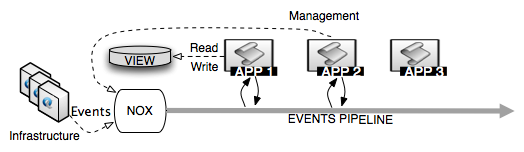
\includegraphics[scale=0.5]{pic/nox-pipeline}
%   \caption[NOX pipeline] {\textbf{NOX pipeline} An overview of the NOX
%     pipeline used for event processing by the Management applications. NOX
%   receives events that have originated either in the Infrastructure of
% the Management layer and dispatches them through a pipeline of
% applications who have registered for processing these events. 
%  As an example: \emph{PACKET\_IN} is a network event while
% \emph{USER\_AUTHENTICATED} could be an application event.}
%   \label{fig:nox-pipeline}
% \end{figure}

% NOX is a component framework with primitives for
% construction and deconstruction of OpenFlow
% based messages. The programming model is event-based. Applications (the components) are registered in a
% priority based pipeline with event handlers associated to either
% OpenFlow or applications events. This process can be seen in Figure
% \ref{fig:nox-pipeline}, which describes the NOX dispatching behavior. Notice
% that applications decide if the event should continue to be processed
% by the pipeline. NOX  currently ships
% with several applications (e.g., forwarding, topology discovery, host
% tracking, spanning tree, layer two switch behavior, etc.).

% NOX is a centralized controller  but the authors argue that it can easily be distributed for resilience if the shared state (the \emph{view}) is consistently distributed. 
% Initially it was a single threaded application not focused on
% performance. However, from its publishing date 
% several improvements have taken place
% \cite{Tootoonchian:2012uia,zen-doc-thesis} that have significantly improved
% NOX performance. Under the set of improvements we highlight the
% natural evolution to a multi-core aware application
% that statically distributes network requests to different threads. 

% In the time of writing, NOX is publicly available but has ramified into
% two different applications: A C++ based controller available in
% Linux and a Python  based controller (POX) available for
% several environments \cite{nox}.

% \subsection{Maestro}

% Maestro is the undergoing work of Zeng Cai covered in
% \cite{maestro}. It is presented as a Network Operating System focused
% in coordination and isolation of the applications  that control the
% infrastructure layer. Cai recognizes that Management components do not
% operate independently and in isolation. Instead, they operate
% concurrently with inter-dependent state (present in the NIB). With this in mind
% it aims to exploit parallell computing benefits in the control plane. 

% Maestro splits the regular pipeline execution such that it can
% be concurrently executed. As seen in Figure \ref{fig:maestro-pipeline} events may
% follow different execution paths since singular control components are
% not interested in every single event. Thus, Maestro can manage to
% execute several applications concurrently. However, in order to
% coordinate the control component access to the NIB Maestro opts to
% have a more granular network state model. The author argues that it is
% common to control components to be  interested only in  subsets of the
% NIB. In order to employ concurrent execution Maestro requires that
% applications specify  what subsets of the NIB they require as input
% and what subsets they modify as output. 

% Maestro employs
% coordination of the  execution of the applications with performance in
% mind. As an example based on Figure \ref{fig:maestro-pipeline} if the routing table
% (subset of the NIB) is updated while the RouteFlow application is running, then
% Maestro makes sure that the application will use the old version of
% the RoutingTable.

% \begin{figure}
%   \centering 
%   \footnotesize
%   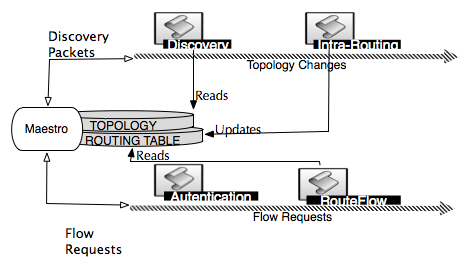
\includegraphics[scale=0.5]{pic/maestro-pipeline.png}
%   \caption[Maestro pipeline]{\textbf{Maestro pipeline} Maestro split the pipeline execution
%   into several concurrent pipelines based on the events applications
%   process and the state they access or modify. In the figure we can
%   see two execution paths: \textbf{Topology Changes} processes the
%   events triggered by changes in the Infrastructure and \textbf{Flow
%     Requests} processes new flow events.}
%   \label{fig:maestro-pipeline}
% \end{figure}


% The fundamental objective of Maestro is to maximize scalability in a
% centralized control plane. To do so it attempts to exploit
% parallelization in the controller server. Three major design goals
% shape Maestro: fair distribution of work across cores; minimal
% overhead introduced by cross-core and cache synchronization and;
% minimal memory consumption. In addition, it also
% exploits throughput optimization through batching. The results
% published show that Maestro linearly scales the throughput with the number of cores
% available on the controller. 


% Currently Maestro is available under the LGPL 2.1 licence. It ships
% with usual switching  and routing capabilities \cite{maestro}.

% \subsection{Beacon}
% \label{sec:beacon}
% Beacon is an open source controller built in Java, by David Erickson during his academic studies in Stanford University. 
% He is, to our knowledge, the only official maintainer of the
% application. 

% Beacon is also a Thin Controller with  an event-based programming model. Applications register for
% specific type of events and process these  in the order
% configured by the user. Any application processing an event chooses to forward the
% event further in the pipeline or terminate its execution. It is also
% multi-threaded, binding switches to particular threads. Applications receive data from all threads.

% Applications in Beacon are implemented as \emph{bundles}. A bundle is the
% unit of abstraction in the OSGI \cite{osgi} framework - a component and service
% platform for the Java programming language with dynamic capabilities -
% allowing features such as \emph{hot-swapping} (i.e., deploy, start and
% stop modules in run time). 
% Beacon provides a central service (the registry) for registration of bundles as
% services. Each bundle implements a service, exports it to the registry and
% other bundles may consume it. Applications events in Beacon take place
% through the service abstraction: bundles may register in other bundles as
% listeners to be notified when for specific events take place. 
% %TODO - reescrever essa ultima frase. 

% Beacon does not provide any NIB service. The network state is
% decentralized and encapsulated in the bundle abstraction. There are
% no persistance  mechanisms also. 

% At the time of writing the applications available are the following: 
%  learning switch, hub, device manager , topology, layer 2
% shortest path routing, arp  proxy, dhcp proxy. 

% %\cite{Controllers: Beacon with David Erickson. Open Network Summit
% %  http://www.youtube.com/watch?v=tZ3G_FDuMjg}

% \subsection{Floodlight}
% Floodlight is an open source Apache licensed controller. It was
% initially forked from Beacon. It  is developed and maintained by an open community of developers that is mainly composed of Big Switch\footnote{A SDN vendor with a commercial
% distributed controller named Big Controller \cite{:vn}.} employers. It is written in Java, but applications can either be
% implemented in Java, Jython or through the REST service
% available in the NOS (with limited functionality). Floodlight is also a Thin Controller. 

% Floodlight follows the common event driven
% programming model of most  controllers. Although Floodlight was originally
% forked from Beacon, the OSGI support was taken for performance and
% deployment reasons. The overall functionality is based on modules
% (i.e., applications) that implement services that can be consumed by
% other modules. It is similar to Beacon in this regard, however the
% module/service functionality is directly provided by Floodlight
% instead of delegated to a third-party framework as OSGI. 

% Floodlight is also multi-threaded. It accomplishes this through an
% asynchronous event based multithreaded library named Netty \cite{netty} that manages Input/Ouput communication with the managed
% switches. 

% Currently the applications available are: topology manager,  link
% discovery, forwarding, device manager, storage, firewall and
% static flow pusher.  


% \section{Distributed Controllers}
% \glsresetall
% \label{sec:relatedWork:distributed}

% In this section we provide an overview of Distributed Controllers
% existent in the literature. By our definition an distributed
% controllers provides explicit support to the deployment of several
% controller processes over one or more servers. 

% \subsection{HyperFlow}
% Motivated by the lack of scalability in centralized controllers, HyperFlow \cite{Tootoonchian:2010vy} 
% was created as a distributed controller. The 
% authors aim was to provide scalability without sacrificing
% the simplicity of management applications  in  centralized controllers. It
% is built as a \emph{C++} application on top of the NOX 
% controller \cite{Gude:2008jd} requiring minor modifications to the
% controller core and is not publicly available. 
% \begin{itemize}
% \item Passively syncrhonizing network-wide views. HyperFlow localizes decision making to individual controllers, thus minimizing the control plane response time to data plane request. 
% \item All controllers share the same eventually consistent view. But no conflicts should arise if the applications respect the rules. 
% \item HyperFlow has the benefit of requiring only minor modifications to existing control applications 
% \item The author point out that controlelrs benefit from having the state locally since request can be served locally. 
% \item Proactively pushes state to other controllers. 
% \item Each controller runs as if they are running the entire network. The HyperFlow application captures commands to switches and responses  and redirects them to the appropriate controllers. 
% \item CRITIC: Under failure it has to replay all events. This can be time consuming and events grow indefinitely. Under this time the controller can not serve requests. If instead this recovery mechanism is isolated from the controllers then a recovered controller (or other in its place) can start processing network events almost immediately. 
% \end{itemize}


% \subsubsection{Architecture.} HyperFlow is composed of two main components: the controller application
% and an event propagation system. The overall architecture can be seen
% in figure \ref{fig:hyperflow-design}. The controller component is
% an application built on top of NOX \cite{Gude:2008jd} which implements an event logger
% responsible for subscribing to OpenFlow events and a command proxy
% capable of sending OpenFlow commands to  network devices. In essence
% HyperFlow interposes  between NOX and
% Management applications. The event
% propagation system allows  communication between HyperFlow
% instances and  is built over a distributed filesystem. Communication
% is done through channels implemented as files. There are three types of channels: the
% control channel where controllers advertise themselves; the data
% channel where general interest events are published by every
% controller;  and finally the individual controller channel for OpenFlow
% commands relevant to the controller who owns the channel. The
% communication system is based on the well known \emph{Publish/Subscribe}
% model  whereby one defines publishers as senders of
% messages and subscribers as the receivers. Publishers do not send
% messages directly  to receivers.  Instead,
% messages are published in a medium (in this case the channels) and
% interested receivers subscribe to publishers through some form of
% subscription logic (e.g., channel, topics, etc.). The Publish/Subscribe
% model allows the decoupling of both space and time in the
% communication between publishers and subscribers. 
% HyperFlow leverages on an existing Publish/Subscribe system that provides: 
% persistent storage of the events published; \emph{FIFO}
% (First-In-First-Out)  ordered delivery of
% the messages published by the same controller; and resilience against
% network partitioning.

% \begin{figure}
%   \centering 
%   \footnotesize
%   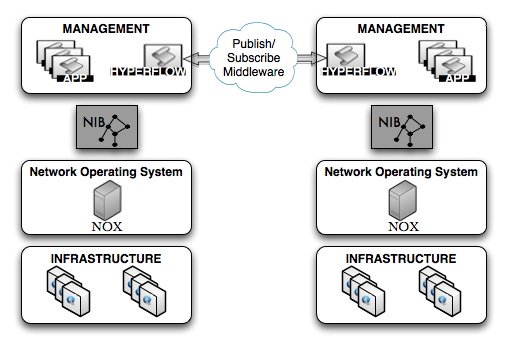
\includegraphics[scale=0.5]{pic/hyperflow-design.png}
%   \caption[HyperFlow architecture]{\textbf{HyperFlow architecture} is  similar to
%     NOX  with the addition of an Publish/Subscribe middleware
%     used between the HyperFlow Management application. The
%     Publish/Subscribe system is used for all communication between controllers.}
%   \label{fig:hyperflow-design}
% \end{figure}


% \subsubsection{State Distribution.} State distribution in HyperFlow is accomplished through the
% Publish/Subscribe event propagation system. The NIB  is
% replicated in all instances and HyperFlow distributes the events
% that cause changes to it. This is done through event publishing in the shared
% data channel. Every controller subscribes to the
% data channel and replays the events received on it, thus changing its
% NIB in a similar way.  The view  is maintained by the Management applications
% residing in the controller and outside the domain of
% HyperFlow (as in NOX). HyperFlow is, in concept,  identical to a \gls{smr} system with the controllers as replicas. State changing events are distributed to all replicas, that execute them to converge to the same state of others. 
% But HyperFlow does not guarantee strong
% consistency as events are not totally ordered  between controllers. 
% Notice that even with FIFO based channels some controller $c$ might receive event $e_i$ followed by event
% $e_j$ sent from controllers $i$ and $j$, while a controller $c'$
% perceives $e_j$ followed by $e_i$. It is possible that such occurrence
% leads controllers to divergent states. The article explicitly adverts
% that Management applications should not rely in event ordering "except
% those targeting the same entity (e.g., the same switch or link)'' as
% those guarantee FIFO ordering. 

% Additionally, Hyperflow  also addresses incorrectness problems caused by
% transient inconsistency across controllers  by defining an
% \emph{authoritative}  controller for each flow. This controller is
% responsible for orchestrating changes in the network regarding some
% flow. As an example, to avoid loop-free forwarding \emph{authoritative}
% controllers are solely  responsible for setting the flow paths across the forwarding
% plane for some specific flow. For this, applications must relay
% requests for some flow to its \emph{authoritative} controller. 

% \subsubsection{Scalability.} HyperFlow addresses scalability of the control plane by minimizing the
% number of events that an instance replicates to others. Thus it is
% focused on the scalability of the CPU and does not address state
% scalability since the NIB is fully replicated in every controller. 

% To minimize the number of events  processed by
% instances, HyperFlow filters the dissemination of events. To this end
% it requires that applications tag locally generated events that affect
% the NIB. Only these events are worth distributing as others are redundant. 

% Local events are generated either by the Management or
% Infrastructure layers but Management applications trigger events as a
% response to the processing of other events (i.e., there is a causality
% relationship between events). Thus, HyperFlow
% minimizes distribution of events even further and if, for example,
% some event $e$ is triggered due to the processing event $i$, it 
% distributes only event $i$. To this end, Management applications
% triggering events have to, both flag the event if it affects the NIB state
% but also to associate the event that caused it. As one single event
% can cause several application events to be triggered this can reduce
% the volume of traffic and processing of redundant events.

% \subsubsection{Programming Model.} Applications running on HyperFlow act as they control the entire
% network. Behind the scenes  HyperFlow redirects requests to the
% network equipment  either to the \emph{authoritative} controller or to the
% controller managing the equipment which the request addresses. The choice depends on the type of
% the request. HyperFlow also routes back  responses to the controller
% responsible for  the request. Also, as previously said, every state
% changing event is seen by every controller. So in the end the NIB of
% the network contains updated information from every  equipment present
% in the network.

% The programming model itself is identical to NOX  (event driven,
% pipeline based) thus
% maintains its simplicity. Some overhead complexity is added as
% HyperFlow requires the applications to tag  state changing events and
% identify parent events as explained above. 

% \subsection{Onix}
% Onix \cite{Koponen:2010th}  was build upon the NOX legacy and
% provides two major contributions: it is the first general controller
% published in the literature, and also the first to provide strong consistency.  Onix 
% provides an improved Network Operating System interface on 
% which the northbound API does not reflect the southbound
% API. Management applications are programmed against a network
% graph of Typed Entities very similar to the Object Oriented paradigm
% and are not aware of the southbound characteristics (e.g., the use of Openflow). The graph is implemented in 
% the \emph{Network Information Base}
% (NIB) and can be distributed across a  cluster of  Onix
% controllers. Applications have the choice to specify consistency and
% durability requirements  per network entity  present in the NIB. 
% Onix was the result of a joint effort between Google, NEC, Nicira,
% ISCI and Berkely, and (at least)  both Google and Ericson have
% developed their controllers based on from Onix \cite{The-Valley-of-the-Nerd.:fk}. At the time of
% writing Onix is not publicly available. 

% \subsubsection{Architecture.} Onix architecture is presented in figure \ref{fig:onix-design}. Only
% one application resides on the 
% Management layer and may communicate with other applications in other
% controllers instances for coordination. The NIB is the
% only element in Onix northbound interface. The Management layer
% directly modifies the NIB and subscribes to changes on it. The Infrastructure layer
% indirectly modifies the NIB (trough the NOS layer). The NOS has to
% guarantee that changes in the Infrastructure are reflected in the NIB
% and vice versa. For this, it translates network events into changes in
% the NIB and changes in the NIB to changes in the Infrastructure configuration. Onix
% supports This process is represented in figure
% \ref{fig:onix-process}.  OpenFlow but it could transparently move to another
% southbound API. 

% Each Onix instance  independently manages a subset of the
% Infrastructure. However the NIB  exposes all the network for each
% instance. As such, each time a local Onix instance alters the NIB these
% changes are reflected in all other instances. Thus, the NIB is also
% the distribution mechanism of the Onix controller. The  distribution
% itself is done by the datastores that back up  the NIB state (seen
% in figure \ref{fig:onix-design}).

% \begin{figure}
%   \centering 
%   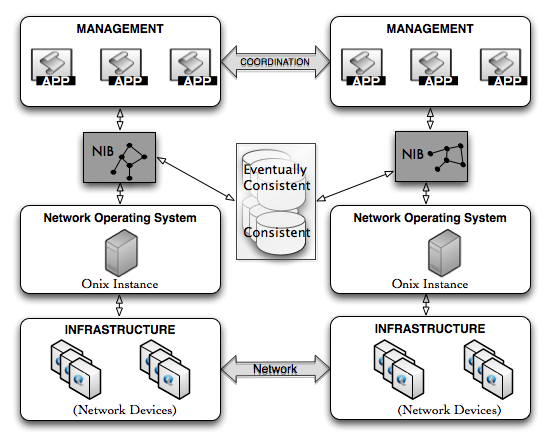
\includegraphics[scale=0.5]{pic/onix-design.png}
%   \caption[Onix architecture] {\textbf{Onix achitecture.} In Onix the NIB is the
%     solely entity used as the northbound api and Managements program
%     directly against it. The NIB is supported by
%     two replicated datastores accessible across Onix instances.  The
%     Management layer communicates across instances for coordination.}
%   \label{fig:onix-design}
% \end{figure}

% \begin{figure}
%   \centering 
%   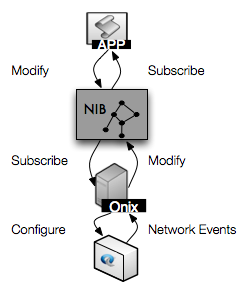
\includegraphics[scale=0.5]{pic/onix-process.png}
%   \caption[Onix configuration process]{\textbf{Onix configuration
%       process}. The interactions between layers of the Onix
%     instance stack. In the figure we can observe the process of
%     configuration on the left side, and the process of detecting
%     changes in the Infrastructure on the right side.\footnote{The Infrastructure should be only one.}} 
%   \label{fig:onix-process}
% \end{figure}

% \subsubsection{State Distribution.} Onix defines a flexible distribution model for the NIB 
% whereby  it offers the application
% designer the choice of consistency guarantees. Two
% replicated datastores are present, covering  strong 
% and  eventually consistency. Strong consistency data is
% provided through a transactional persistent database backed up by a replicated
% state machine. This datastore is
% favored for data with low-frequency changes  as its performance limitations are
% significant. The eventually consistent datastore consists in 
% an one hop memory based DHT  (as Dynamo 
% \cite{DeCandia:2007cn}) favored for  volatile data with high update
% rates. 

% The NIB reflects the state of both datastores. Both the integration of
% datastores and the inconsistency  characteristics of the DHT can lead the
% NIB to an inconsistent state where reads performed in some entity may
% return more than one result. Thus Onix provides primitives
% for the integration of inconsistency resolution logic as well as 
% direct integration of a distributed
% coordination framework (see  ZooKeeper \cite{Hunt:2010ux}) in the
% northbound interface. 

% \subsubsection{Scalability.} Onix is intended for large scale Infrastructure where scalability is
% fundamental. In each Onix instance the NIB
% size reflecting the network state could lead to memory
% exhaustion   and the processing of both network events and
% subscriptions 
% to changes in  the NIB can lead to CPU exhaustion.

% In order to introduce scalability and avoid exhaustion, partition and
% aggregation based techniques can be configured in the Management
% layer. Partition avoids full replication of both data  and workload
% such that additional instances do not only replicate overall work but
% also relief it. As for aggregation it can, for example, allow network entities to be
% aggregated and exposed for other Onix instances as only one.

% In practice partition in Onix is present in the division of the
% Infrastructure across different Onix instances. 
% This way
% instances process fewer events. Additionally the Management logic can
% configure Onix instances to keep only subsets of the NIB in memory and
% up to date. For aggregation, an Onix instance can be configured to
% expose a subset of the NIB as an aggregated element. 

% \subsubsection{Programming Model.} Applications are built against the NIB graph data structure that is
% composed of \emph{Typed Entities} supporting the Object
% Oriented paradigm (i.e., encapsulation of data, functions over
% entities, hierarchy, etc.). Onix supports extensible representations of
% network entities. The
% API provides essential functions to search, inspect, create, destroy and
% modify entities present in the NIB. It is also possible to register
% notifications for creation, removal and updates of data
% entities. When network events of other Onix instances update the
% datastores those changes must be reflected on the local NIB and the
% application must be notified through a callback function. 
% All operations are asynchronous, with
% eventual delivery and no ordering or latency guarantees given
% therefore a \emph{barrier} synchronization primitive is available
% allowing the application to wait as
% updates are translated and applied in the network devices and/or other
% controllers. 

% Finally it is worth mentioning that Onix employs coarse-grained
% locking mechanisms over the NIB. Applications are given the guarantee
% that no other local thread concurrently updates the NIB. 

% \subsection{Kandoo}
% Kandoo \cite{Yeganeh:2012jm} is an hierarchical controller for
% scalable infrastructures. The main
% contribution comes from the deployment of isolated controllers near
% the switches that shield a parent  controller from processing all
% events originating at the network. It is implemented in a mixture of
% C, C++ and Python and is not publicly available. 

% \subsubsection{Architecture.} In Kandoo --- see Figure  \ref{fig:kandoo-design} --- the controller is split in two levels: in the top level (Network Operating System layer) we
% have the root controller responsible for normal operation. In the
% bottom (at the Infrastructure layer) we have local controllers that are (ideally)  closer to the
% managed switches. This two level design allows  shielding the
% controller from frequent events triggered by 
% the network devices. Notice that  the entire SDN
% stack is replicated in the Infrastructure with the exception of the
% NIB since the bottom Management layer should not require direct access to the NIB services. If necessary access to NIB
% must be directed to the root controller.

% \begin{figure}
%   \centering 
%   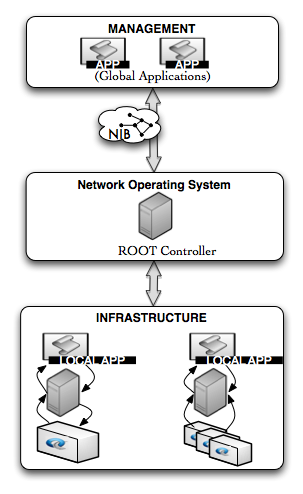
\includegraphics[scale=0.5]{pic/kandoo-design.png}
%   \caption[Kandoo design] {\textbf{Kandoo design.} Kandoo decomposes the usual controller
%     design into two layers. For this, it brings both controllers and
%     applications closer to the Infrastructure. The controllers
%     residing in the Infrastructure layer are responsible for
%     processing frequent events that do not require access to the
%     network state present at the NIB.} 
%   \label{fig:kandoo-design}
% \end{figure}

% This design is motivated by the ideia of bringing control
% functionality towards the datapath. As such, \emph{Local Apps} should
% require no network wide state and the bottom controllers should stay
% close to switches. The deployment of the bottom control plane can
% even happen directly at the switches if they support this
% functionality (e.g., software switches). 

% The remaining design of the controller is not well specified in the
% paper. However, other architectures can complement the Kandoo architecture.
% The authors stress that even distributing the root
% control plane through Onix or HyperFlow is orthogonal to the remaining design.

% \subsubsection{Scalability.} In Kandoo scalability is supported by the introduction of the two
% level hierarchy. The bottom control plane  shields the root
% control from processing of events. As the bottom plane does not
% requires access to the NIB it remains simple and
% efficient. Additionally, as it is closer to the data plane latency
% penalties are lower. However the effectiveness of this
% scalability mechanism depends on the Management functionality. For
% effective shielding one requires Management applications capable of
% operating without access to the network state. The article does not
% specifies how practical or significant are this class of
% applications beyond exemplifying local policy enforcement  and the
% Link Layer Discovery Protocol. 

% \subsubsection{Programming Model.} In Kandoo the NOS layer is responsible for the deployment of local
% applications in the bottom control plane. The application model only
% requires that the applications deployed at the NOS have a flag
% that sets its scope (i.e., local or non-local). All the remaining work
% is left for the root controller. 

% % \subsection{Comparison to Blah, Critic}
% % This section is only a scratch for future work orientation. It is
% % intended as a comparison to the use of the NIB we are going to build
% % and also to criticize the limitations and problems of both HyperFlow
% % and Onix. 
% % \begin{description}
% % \item[TODO] make it clear that HyperFlow replicates controllers. 
% % \item[Scalability in Onix] It doesn't exist in the published work (By
% %   now it should exist off course). There is quite a bit of blah in the
% %   paper about techniques and such but in reality all is left for the
% %   application layer to implement relying (again!) on distributed
% %   coordination and locking mechanisms; 
% % \item[Strong consistency in Onix] Not 100 \% sure about this: it does
% %   not exist in practice. If an application mixtures Strong consistency
% %   nodes with eventually consistent  links (i.e., (Object A is strong consistent and
% %   contains B eventual consistent) it must be prepared to deal
% %   with inconsistent resolution upon dealing with the node. The paper
% %   suggests this. It is
% %   overly complicated in the application logic. 100 \% strong
% %   consistency simplifies a lot the application development. 
% % \item[Typed entities, Nib Abstraction in Onix] Really cool. higher
% %   level of abstraction, another level of indirection. Typed entities
% %   combined with the NIB is eternal code loosely coupled to management
% %   protocols used in the management of network equipment. Casado
% %   defends in a network post
% %   [http://networkheresy.com/2011/08/09/what-might-an-sdn-controller-api-look-like-and-should-we-standardize-it/]
% %   that it is a general loosely coupled layer, independent of the state
% %   distribution mechanism. I disagree, at least in the published
% %   work. The state distribution is ``à vista'' in the application layer
% %   (define consistency per entity, conflict resolution). It is not
% %   fully transparent and consequently not loosely coupled. 

% % \item[HyperFlow concept] Kind of reminds a distributed state machine
% %   at application level (replay all relevant controller events -i.e.,
% %   state changing events) but lacks ordering requirements. 

% % \item[HyperFlow] favors availability over consistency. O nosso não
% %   fará isso. 
% % \item[HyperFlow] sucks. guarantees a bounded window of inconsistency
% %   if the network changes trigger less than around 1000 events per
% %   seconds. 
% % \item[Onix] allows both. The Management deciding. Sacrificing
% %   transparency, simplicity. Also, it sucks. 

% % \item[Resumo] Hyerflow distribui os eventos o que e estupido porque há
% %   muito mais eventos que alteracoes na NIB. Então ele distribui só os
% %   eventos que mudam a NIB. O Onix oferece os dois tipos de coerencia
% %   mas complica a programacao porque Entities que combinam dois tipos de
% %   coerencia podem sempre retornar dois resultados. O Kandoo mete
% %   hierarquia ao barulho para minimizar o numero de eventos. 


% % \end{description}

% \section{Consistent Data Stores}
% \glsresetall
% \label{sec:relatedWork:consistentDataStore}
% %explain 2f+1. 
% %Section data stores do artigo. 
% The key idea of our controller architecture is to make the controller instances coordinate their actions through a dependable data store in which all relevant state of the network and of its control applications is maintained in a consistent way.
% This data store is implemented with a set of servers (replicas) to avoid any single point of failure, without impairing consistency.
% One of the most popular techniques for implementing such replicated data store is state machine replication (SMR)~\cite{Sch90,Lam98}.
% In this section we review the state of the art on replicated data stores and describe some reasons why, contrary to common belief, they can be a valid option for supporting a distributed controller architecture.

% Practical crash fault-tolerant replicated state machines are usually based on the Paxos agreement algorithm for ensuring that all updates to the data store are applied in the same order in all replicas (thus ensuring consistency)~\cite{Lam98}.
% Since the original Paxos describes only an algorithmic framework for maintaining synchronized replicas with minimal assumptions, we instead describe the Viewstamped Replication (VR) protocol, a similar (but more concrete) state machine replication algorithm introduced at the same time~\cite{reitblatt2012abstractions}.
% Fig. \ref{fig:paxos} shows the messages exchanged in Paxos/VR for an update operation: the client sends a message to a primary replica (the leader) that disseminates the update to all other replicas. These replicas write the update to their log and send an ACK to the primary.
% In the final step the leader executes the request and sends the reply to the client.
% If the primary fails, messages will not be ordered and thus a new primary will be elected to ensure the algorithm makes progress.
% When read-only operations are invoked, the leader can answer them without contacting the other replicas.
% Strong consistency is ensured due to the fact that all requests are serialized by the leader.

% \begin{figure}[!ht]
% \centering
% \includegraphics[width=0.5\textwidth]{pic/related/vr.pdf}
% \caption[Paxos/VR update protocol]{Paxos/VR update protocol.} 
% \label{fig:paxos} 
% \end{figure}

% The Paxos/VR algorithm has served as the foundation for many recent replicated (consistent and fault-tolerant) data stores, from main-memory databases with the purpose of implementing coordination and configuration management (e.g., Apache'  Zookeeper~\cite{Hun10}), to experimental block-based data stores or virtual discs~\cite{Rao11,Bol11,Bes13}, and even to wide-area replication systems, such as Google Spanner~\cite{Corbett:2012uz}.
% Besides the synchronization protocol, these systems employ many implementation techniques to efficiently use the network and storage media.

% Although not as scalable as a weakly consistent data store, these systems grant the advantages of consistency for a large number of applications, namely those with moderate performance and scalability requirements. To give an idea of the performance of these systems, Table \ref{table:smr-results} shows the reported throughput for read and write operations of several state-of-the-art consistent data stores.

% \begin{table}
%   \center
%     \begin{tabular}{ lccc}
%     \hline
%     \emph{System} & \emph{Block Size} & \emph{kRead/s} & \emph{kWrite/s} \\ \toprule
%     Spanner \cite{Corbett:2012uz} & 4kB & 11 & 4 \\ 
%     Spinnaker \cite{Rao11} & 4kB & 45+ & 4 \\  
%     SCKV-Store \cite{Bes13} & 4kB & N/R & 4.7 \\ 
%     Zookeeper \cite{Hun10} & 1kB & 87 & 21 \\ \bottomrule 
%     \end{tabular}
%   \caption[Performance of state machine replication systems]{Throughput (in thousands data block reads and writes per second) of consistent and fault-tolerant data stores based on state machine replication (N/R = Not Reported).}
%   \label{table:smr-results}
% \end{table}

% Given the differences in the design and the environments where these measurements were taken, we present these values here only as supporting arguments for the possibility of using consistent data stores for storing the relevant state of SDN control applications.
% Depending on the specific application this state may include, for instance, a subset of the Network Information Base (NIB).
% Interestingly, these values are of the same order of magnitude of the reported values for \emph{non-consistent} updates in Onix (33k small updates per second considering 3 nodes~\cite{koponen2010}), and much higher than the reported values for their consistent data store (50 updates/second for transactions with a single update).
% The Onix paper does not describe how its consistent database is implemented but, as shown by these results, its performance is far from what is being reported in the current literature.


% \section{Consistent Data Planes}
% \glsresetall
% \label{sec:relatedWork:consistentPlane}


% Recent work on SDN has explored this need for consistency at different
% levels. Programming languages such as Frenetic~\cite{Foster2011} offer
% consistency when composing network policies (automatically solving
% inconsistencies accross network applications' decisions). Other
% related line of work~\cite{reitblatt2012abstractions} proposes
% abstractions to guarantee data-plane consistency during network
% configuration updates. The aim of these systems is to guarantee
% consistency \textit{after} the policy decision is
% made. Onix~\cite{Koponen:2010:ODC:1924943.1924968} provides a
% different type of consistency: one that is important \emph{before} the
% policy decisions are made. Onix provides network state consistency ---
% both weak and strong --- between different controller instances. The
% datastore we propose is similar in that it offers strong consistency
% for network (and application) state between controllers\footnote{By
%   strong consistency we mean that all accesses to the datastore are
%   seen by all controller instances in the same order
%   (sequentially).}. Our main objective is to improve the ``performance
% limitation''~\cite{Koponen:2010:ODC:1924943.1924968} of Onix's
% transactional persistent database. 


% Other works on SDN consistency include the Frenetic programming language~\cite{Foster2011}, Reitblatt et al. work on abstractions for network update~\cite{reitblatt2012abstractions}, and Software Transactional Networking~\cite{Canini:2013:HotSDN:STN}. 
% These papers address different consistency issues, however. 
% In essence, they target consistent flow rule updates on switches, dealing with overlapping policies and using atomic-like flow rule installation in SDN devices.
% In other words, they take care of data-plane consistency \emph{after} the policy decisions are made by the network applications. 
% Frenetic offers a high level language and a run-time system that, besides other benefits, ensures that policy rules made by concurrent network applications are not overlapped, thus avoiding network inconsistencies.
% In~\cite{reitblatt2012abstractions} the authors propose two abstractions --- per-packet and per-flow consistency --- and mechanisms to guarantee that on a network update a packet (or a flow) is processed by exactly one consistent global network configuration. 
% STN extends these works by proposing a transactional solution to provide consistent rule installation in a distributed setting. 
% Our work targets consistency at a different level.
% Our datastore ensures strong control-plane consistency for network
% and/or applications state, which means policy decisions are always
% based on a consistent state.


%%% Local Variables: 
%%% mode: latex
%%% TeX-master: "../PEI"
%%% End: 
